% !TeX root = ./jvk-blatt1.tex

\newcommand{\jvkpackage}{MatrixJVK.zip}
\newcommand{\jvkpackageurl}{http://hier.placeholder.web/file}

\excercise{Programmstart}

\begin{Infobox}[HowTo: Wie bekomme ich des Projekt]
    \begin{enumerate}
        \item Lade als erstes das Maven-Projekt \jvkpackage runter, man findet es hier:
        \begin{center}
            \color{blue}\href{\jvkpackageurl}{\textit{\jvkpackageurl}}
        \end{center}

        \item Nachdem das Zip-File runter geladen ist muss man es in einem geeigneten Ordner entpacken.\\
        \textbf{Windows:} Entpacken funktioniert durch einen Rechtsklick auf die Datei und dann durch klick auf \fbox{Alle extrahieren...}$\to$\fbox{Extrahieren}.\\
        \textbf{Linux:} Am schnellsten enpackt man ein Zip-File übers Terminal mit dem Befehl:
        \newline\hspace*{\fill}\texttt{\textgreater\ unzip \jvkpackage}\hspace*{\fill}\newline
        \textbf{Apple:} Nachdem man das Zip-File im Finder offen hat entpackt man es durch einen einfachen Doppelklick.
    \end{enumerate}
\end{Infobox}

\begin{Infobox}[HowTo: Projekt Import in Eclipse]
    \begin{enumerate}
        \item Um ein Projekt zu importieren klicke zuerst auf \fbox{File} $\to$ \fbox{Import...}.
        \item Wähle in dem Ordner \fbox{Maven} $\to$ \fbox{Existing Maven Projects} oder nutze das Suchfeld oben um \fbox{Existing Maven Projects} zu finden. Klicke dann auf \fbox{Next \textgreater}.
        \item Drücke oben rechts auf \fbox{Browse...} und suche das Verzeichnis, wo die Datei \jvkpackage entpackt wurde.
        \item Stelle sicher das der Projekt Name im \textit{Projects} Bereich des Fensters auftaucht.
        \item Zu guter letzt noch auf \fbox{Finish} drücken.
        \item Nachdem sich das Fenster geschlossen hat, siehst du das Projekt im \textit{Package Explorer} links an der Seite.
        \item Das euer Projekt richtig funktioniert solltet ihr im \textit{Package Explorer} das Projekt mit einem Rechtsklick auswählen und dann im Kontextmenü \fbox{Maven} $\to$ \fbox{Update Project...} $\to$ \fbox{OK} ausführen.
    \end{enumerate}
\end{Infobox}

\newpage

Öffne nun die Entwicklungsumgebung Eclipse und importiere das heruntergeladene Maven-Projekt \jvkpackage wie oben in den beiden HowTo's beschrieben.

\begin{enumerate}[label=\alph*)]
    \item Führe das Projekt aus, es sollten keine Fehler auftauchen aber auch nichts passieren.
    Wir haben ja auch noch nichts programmiert.
    \item Finde die \texttt{Main} Klasse und füge dort folgenden Code ein.
    Aktuell musst du den Code noch nicht verstehen, es geht hier mehr darum sich in Eclipse zurecht zu finden.\\
    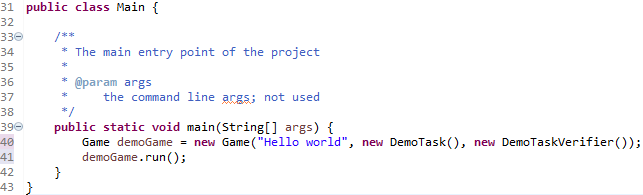
\includegraphics[width=\linewidth]{./figures/code.1.png}\\
    Wenn der Code jetzt ausgeführt wird geht ein Fenster auf mit der Simulator Ansicht.
    Suche nun die Stop Taste in Eclipse um das Programm abzubrechen.
    Du findest sie in Eclipse unten bei der Console.
    \item Versuche nun den Code so zu verändern das dein Name im Fenster Titel steht.
\end{enumerate}

\begin{Infobox}[HowTo: Auskommentieren]
    Manchmal möchten wir, dass bestimmter code nicht ausgeführt wird, aber wir wollen das er später wieder ausgeführt wird oder möchten ihn einfach nicht verlieren.
    In diesen Fällen Kommentieren wir die Code Zeile einfach aus.
    Dies geht indem wir der Code Zeile zwei Schrägstriche ({\color{javagreen}\texttt{//}}) vorran stellen.
    Als Beispiel betrachten wir folgenden Code.

    \begin{lstlisting}
public void run(Simulation sim) {
    PlayfieldModifier pm =
            new PlayfieldModifier(sim.getPlayfield());
    pm.placeEntityAt(new Coin(), new Position(0, 0));
}
    \end{lstlisting}

    Wenn wir nun die letzte Zeile 'ausschalten' wollen stellt sich der Code wie folgt dar.

    \begin{lstlisting}
public void run(Simulation sim) {
    PlayfieldModifier pm =
            new PlayfieldModifier(sim.getPlayfield());
    //pm.placeEntityAt(new Coin(), new Position(0, 0));
}
    \end{lstlisting}

    Denn alles ab den zwei Schrägstrichen bis zum Zeilen Ende wird nun 'ignoriert' was durch eine andere Färbung in Eclipse deutlich wird.
\end{Infobox}

\begin{enumerate}[label=\alph*)] \setcounter{enumi}{3}
    \item Finde herraus was passiert wenn man die erste oder die zweite Zeile in der Main-Funktion auskommentiert.\\
    Hinweis: NIcht alle Varianten kompilieren zwangsläufig, überlege warum das sein könnte.
    \item Finde eine Möglichkeit den Fenster Titel nach der \texttt{demoGame.run();} Zeile zu ändern.
    \item Optional: Versuche drei Fenster gleichzeitig zu starten.
    %\item Optional:  Eclipse funktionen manuell triggern (autocomplete [strg + leer], autoformat [strg + shift + f], Javadoc on hover, run, debug [und wie man wieder in die java view kommt], package explorer bedienen, rückgängig [strg+z], umbenennnen von variablen [f2])
\end{enumerate}
